This chapter will introduce the \emph{\index{Fourier series}{Fourier
series}}, which is used to express a periodic signal as a sum of
sinusoidal signals. This is the first time that a spectral
representation of signals is introduced. We will explore the following
topics:
\begin{itemize}
  \item Signals as a sum of sinusoids.
  \item Periodic signals, \emph{\index{fundamental frequency}{fundamental frequency}} and \emph{\index{fundamental period}{fundamental period}}.
  \item Expressing a periodic function as a sum of complex sinusoidal signals (Fourier series \index{synthesis}{synthesis}).
  \item Determining the phase and amplitude of each Fourier series coefficient (Fourier series \index{analysis}{analysis}).
  \item Derivation of the \emph{\index{continuous-time Fourier transform}{continuous-time Fourier transform}} as a generalization of the Fourier series.
\end{itemize}

\begin{marginfigure}
  \begin{center}
    \begin{tikzpicture}
      \begin{axis}[
          width=7cm,
          height=6cm,
          ymin=-.8,
          xmin=-3,
          ymax=1.8,
          xmax=3,
          yticklabels={,,},
          xtick={-2,-1.5,-1,-0.5,0,0.5,1.0,1.5,2},
          xticklabels={,,},
          %       legend pos=outer north east,
          xlabel=$\omega$,
          ylabel=$\hat{x}(\omega)$,
          axis lines = middle]
        % real
        %   \addplot +[dirac,blue] coordinates {(1,1)};
        \addplot+[dirac,color=blue,mark options={blue}] plot coordinates {(-2,0.5) (0.5,1.4) (2.5,0.6)};
        %   \addlegendentry{$\mathrm{Re}\{c_k\}$};
        % imag
        %   \addplot+[ycomb,color=red,mark=*,mark options={red}] plot coordinates {(0.5,-0.5) (1.0,-1.0) (1.5,1.3) (2,-0.1)};
        %   \addlegendentry{$\mathrm{Im}\{c_k\}$};

        %  \addplot+[ycomb] plot coordinates {(-0.5,1) (-1.0,0.8) (-1.5,1.3) (-2,0.5)};
        %   \addplot+[ycomb,color=brown] plot coordinates {(0.0, 1.4)};

        \node at (axis cs:-2.0,0.5) [above, font={\footnotesize}]{$c_1$};
        \node at (axis cs:0.5,1.4) [above, font={\footnotesize}]{$c_2$};
        \node at (axis cs:2.5,0.6) [above, font={\footnotesize}]{$c_N$};

        \node at (axis cs:-2,-.4) [below]{$\omega_1$};
        \node at (axis cs:0.5,-.4) [below]{$\omega_2$};
        \node at (axis cs:2.5,-.4) [below]{$\omega_N$};

        \node at (axis cs:1.5,1.0) [below]{$\cdots$};


      \end{axis}
    \end{tikzpicture}
  \end{center}
  \caption{A spectral representation of a signal consisting of $N$ complex sinusoidal signals.
    It is not a coincidence that I'm using the same arrow symbol here that I used earlier when introducing the Dirac delta function.}
  \label{fig:spec_rep}
\end{marginfigure}

\newthought{Here is a signal represented as a sum of complex sinusoidal signals}:
\begin{equation}
  x(t) = \sum_{k=1}^N c_k e^{i\omega_k t} \,\,.
  \label{eq:general_spectrum}
\end{equation}
The symbol $c_k = A_k e^{i\phi_k} \in \mathbb{C}$ is used for complex-valued constants that contain information about the
amplitudes $A_k \in \mathbb{R}_{\ge 0}$ and phases $\phi_k \in \mathbb{R}$ of the complex exponential
signals with angular frequencies $\omega_k \in \mathbb{R}$.

It is possible to plot the complex coefficients $c_k$ as a function of angular frequency $\omega$ as
shown in Figure \ref{fig:spec_rep}, which depicts a function of the form:
\begin{equation}
  \hat{x}(\omega) = \sum_{k=1}^N c_k \delta(\omega - \omega_k) \,\,.
  \label{eq:freq_deltas}
\end{equation}
This is a spectral or frequency domain representation of the signal described in Equation \ref{eq:general_spectrum}.
In this case, one can think of the spectrum as consisting of infinitely narrow spectral lines,
each defined by complex constants $c_k$ that are located at angular frequencies $\omega_k$.
We will derive Equation \ref{eq:freq_deltas} later when discussing the continuous-time Fourier transform.

\newthought{A spectral representation of a cosine signal} consists of two frequency components.
One with a positive and one with a negative frequency. This is a direct consequence of Euler's formula.

\begin{marginfigure}
  \begin{center}
    \begin{tikzpicture}
      \begin{axis}[width=7cm,height=5cm,ymin=-1,xmin=-2,ymax=1.8,xmax=2,  yticklabels={,,},
          xtick={-1, 1.0},
          xticklabels={$\omega_{-1}$,$\omega_1$},
          xlabel=$\omega$, axis lines = center]
        % re
        \addplot+[ycomb,color=blue,mark=*,mark options={blue}] plot coordinates {(1,1)};
        % im
        \addplot+[ycomb,color=red,mark=*,mark options={red}] plot coordinates {(1,0.5)};
        % re
        \addplot+[ycomb,color=blue,mark=x,mark options={blue}] plot coordinates {(-1,1)};
        % im
        \addplot+[ycomb,color=red,mark=x,mark options={red}] plot coordinates {(-1,-0.5)};

        \node at (axis cs:1,1.1) [above, font={\footnotesize},mark=none]{$\frac{A}{2}e^{i\phi}$};
        \node at (axis cs:-1,1.1) [above, mark=none, font={\footnotesize}]{$\frac{A}{2}e^{-i\phi}$};
      \end{axis}
    \end{tikzpicture}
  \end{center}
  \caption{A spectral representation of a cosine signal consists of two frequency components:
  $\frac{1}{2}Ae^{i\phi}e^{i\omega t}$ and $\frac{1}{2}Ae^{-i\phi}e^{-i\omega t}$.
  Here $A$ is a non-negative real-valued amplitude. Blue denotes the real and the red denotes the imaginary component of $c_k$.}
  \label{fig:exspecsin}
\end{marginfigure}

Consider the following signal:
\begin{equation}
  x(t)=A\cos(\omega t+\phi) \,\,,
\end{equation}
where $A\in \mathbb{R}_{\ge 0}$. We can use Euler's formula to obtain the spectral representation:
\begin{align}
  x(t) & = \frac{A}{2}e^{i\phi}e^{i\omega t} + \frac{A}{2}e^{-i\phi}e^{-i\omega t} \\
       & = c_1 e^{i\omega_1 t} + c_{-1} e^{i\omega_{-1} t}                         \\
       & = \sum_{k\in\{-1,1\}} c_k e^{i\omega_k t} \,\,.
\end{align}
The second line is simply representing the first line in the format of Equation \ref{eq:general_spectrum}.

Note that there is symmetry within the frequency components. The pairing of frequencies exists as $\omega_{1}=-\omega_{-1}$.
The complex constants are also conjugate symmetric $c_{-1} = c_{1}^*$. We'll later on see
that this type of conjugate symmetry exists for the frequency components of all real-valued signals.

\newthought{A Fourier series is a spectral representation of a signal where each frequency
  is a multiple of some common base frequency $\omega$}:
\begin{equation}
  x(t) = \sum_{k=1}^N c_k e^{i \omega_k t} = \sum_{k=1}^N c_k e^{i \ell_k \omega t} \,\,.
  \label{eq:fourier_series_0}
\end{equation}
Here $\ell_k \in \mathbb{Z}$ is integer valued. If we compare Equation \ref{eq:fourier_series_0} with
the first definition of a spectral representation in Equation \ref{eq:general_spectrum}, we can see
that all angular frequencies are integer multiples of a positive valued angular
base frequency $\omega \in \mathbb{R}_{\ge 0}$:
\begin{equation}
  \omega_k = \ell_k\omega \,\,.
  \label{eq:integer_multiple}
\end{equation}
The largest possible value $\omega$ is called
the \emph{\index{fundamental angular frequency}{fundamental angular
frequency}} of the signal. 

The \emph{\index{fundamental period}{fundamental period}} $T$ of the
signal is related with the fundamental angular frequency $\omega$ as
follows:
\begin{equation}
  \boxed{
    T = \frac{2\pi}{\omega}
  } \,\,.
  \label{eq:fundamental_period}
\end{equation}

The definition of periodicity for a function is that the following condition is satisfied:
\begin{equation}
  \boxed{
    x(t) = x(t+T)
  } \,\,.
\end{equation}
It is relatively easy to show that periodicity follows from the
definition of the Fourier series, by inspecting the periodicity of
each frequency component separately:
\begin{equation}
  c_k e^{i \ell_k \omega t} = c_k e^{i \ell_k \omega (t+T)} = c_k e^{i (\ell_k \omega t+ 2\pi \ell_k )} = c_k e^{i \ell_k \omega t} \,\,.
\end{equation}
We have used the definition of $T$ in
Equation \ref{eq:fundamental_period}. Because all frequency components
are periodic signals with period $T$, it follows that the sum of all
frequency components is periodic as well.

\begin{marginfigure}[0cm]
  \begin{center}
    \begin{tikzpicture}
      % \begin{pgfinterruptboundingbox}
      \begin{axis}[width=1.5\textwidth, height=30em,
          %	title={Discrete-time signal},
          axis x line=center,
          axis y line=middle,
          xmax=0.8,
          xlabel=$t$,
          xticklabels={,,},
          yticklabels={,,},
          ymax=3.0,
          ylabel=$x(t)$]

        \addplot[domain=-0:0.666666667,samples=200,color=blue] {cos( deg(2*3.1415*9*x))-
          cos( deg(2*3.1415*15*x))};
        \addplot[domain=-0:0.666666667,samples=200,color=red] {sin( deg(2*3.1415*9*x))-
          sin( deg(2*3.1415*15*x))};

        \node at (axis cs:0.16666667,2.5) {$\displaystyle{T}$};
        \addplot [dimen] plot coordinates {(0,2.3) (0.33333,2.3)};
        \node at (axis cs:0.33333333+0.16666667,2.5) {$\displaystyle{T}$};
        \addplot [dimen] plot coordinates {(0.33333,2.3) (0.6666667,2.3)};

      \end{axis}
      %\end{pgfinterruptboundingbox}
      %\draw[use as bounding box] ([xshift=0cm,yshift=0cm]current axis.south west) 
      %    rectangle ([xshift=0cm,yshift=0cm]current axis.north east);
    \end{tikzpicture}
  \end{center}
  \caption{Periodic function $e^{i 2\pi 9t} - e^{i 2\pi 15t}$. 
  Blue denotes the real and red denotes the imaginary component of the signal.}
  \label{fig:ex_periodic}
\end{marginfigure}

A consequence of Equation \ref{eq:integer_multiple} is that the ratios
of all pairs of angular frequencies $\omega_k$ and $\omega_{\ell}$ in
Equation \ref{eq:general_spectrum} need to be rational numbers. In
other words, it must be possible to express them in the following form
\begin{equation}
  \frac{\omega_k}{\omega_{\ell}} = \frac{n}{m} \in \mathbb{Q} \,\,
\end{equation}
in order for the signal to be periodic. Here $n$ and $m$ are arbitrary
integers and $k$ and $\ell$ are all unique combinations of the
frequency indices.  If the ratio of two real numbers
$\omega_1,\omega_2\in\mathbb{R}$ is a rational number
$\omega_1/\omega_2 \in \mathbb{Q}$, the numbers $\omega_1$ and
$\omega_2$ are called \emph{\index{commensurable}{commensurable}.}
All angular frequencies for a Fourier series need to be commensurable
relative to one another in order for the signal to be periodic.

How does one determine the fundamental frequency $\omega$? It is
possible to apply \emph{\index{Euclid's algorithm}{Euclid's
algorithm}}. This is sometimes referred to as
the \emph{\index{greatest common divisor}{greatest common divisor}}
for the set of frequencies $\omega_k$. Note that this algorithm will
only produce a result in a finite number of steps if the set of
numbers $\{\omega_k\}$ are commensurable!

\newthought{Here is an example}. Let us assume that a signal is defined as
\begin{equation}
  x(t) = c_1 e^{i \omega_1 t} + c_2 e^{i \omega_2 t} = e^{i 2\pi 9t} -
  e^{i 2\pi 15t} \,\,.
\end{equation}
Is this signal periodic? If so, what is its fundamental frequency
$\omega$ and fundamental period $T$?

In order for this signal to be periodic, $\omega_1$ and $\omega_2$
must be commensurable.  In other words,
$\omega_1/\omega_2 \in \mathbb{Q}$. This is the case, as it is clear
that $\omega_1/\omega_2 = 3/5$ is a rational number.

This signal has two unique angular frequencies: $\omega_1 = 2\pi 9$
and $\omega_2 = 2\pi 15$.  Let's use Euclid's algorithm\sidenote{The
general principle behind the algorithm is that if $\omega_1
= \omega \ell_1$ and $\omega_2=\omega \ell_2$ with $\ell_1$ and
$\ell_2$ integers, then $\omega_1 - \omega_2 = \omega(\ell_1-\ell_2)$
is still divisible with $\omega$.} on these two numbers to determine
the fundamental angular frequency $\omega$.  We start with the two
numbers: $(2\pi 9, 2\pi15)$. Then subtract the smallest number from
the largest number $2\pi 15 - 2\pi 9 = 2\pi 6$ and replace the larger
number with the remainder: $(2\pi 9, 2\pi 6)$.  We repeat this process
until both numbers are the same.  All the iterations are shown below:
\begin{align*}
  (2\pi 15, 2\pi 9)        &                     \\
  (2\pi 15-2\pi 9, 2\pi 9) & = (2\pi 6, 2\pi 9)  \\
  (2\pi 6, 2\pi 9-2\pi 6)  & = (2\pi 6, 2\pi 3)  \\
  (2\pi 6-2\pi 3, 2\pi 3)  & = (2\pi 3, 2\pi 3).
\end{align*}
And we thus find that the fundamental frequency is $\omega=2\pi 3$ and, using
Equation \ref{eq:fundamental_period}, we find that $T = 1/3$.

\begin{marginfigure}[1cm]
  \begin{center}
    \includegraphics[width=\textwidth]{ch01/figures/fourier_head.jpg}
  \end{center}
  \caption{Jean-Baptiste Joseph Fourier}
  \label{fig:joe_fourier2}
\end{marginfigure}

\newthought{The Fourier series is a spectral representation of a periodic function} and is defined as
\begin{equation}
  \boxed{
    x_N(t) = \sum_{k=-N}^{N} c_k e^{i \frac{2\pi}{T} k t}
    \label{eq:synthesis_eq}
  } \,\,.
\end{equation}
The fundamental period of a periodic signal is related to the fundamental angular frequency
as follows: $T=2\pi/\omega$.
We can turn this around and express the fundamental angular frequency as a function of
the fundamental period $\omega=2\pi/T$, as we have done above.


This Fourier series is named after Jean-Baptiste Joseph Fourier
(1768–1830).  He introduced this representation for the purpose of
solving the heat equation using a series of sinusoidal characteristic
solutions. Perhaps the most revolutionary outcome of his study was
that a wide range of functions can be represented as a sum of
elementary sinusoidal functions.

Given a set of Fourier series coefficients $c_k$, we can synthesize a
signal $x_N(t)$.  This procedure is
called \emph{\index{synthesis}{synthesis}}.  This formula shown in
Equation \ref{eq:synthesis_eq} is also called the Fourier series
synthesis equation.\sidenote{Synthesis: \begin{equation*}c_{-N},c_{-N+1},\cdots,c_{N} \rightarrow x_N(t)\end{equation*}\\Analysis: \begin{equation*}x(t) \rightarrow c_{-N},c_{-N+1},\cdots,c_{N}\end{equation*}}

The inverse operation, determining coefficients $c_k \in \mathbb{C}$ from a certain
periodic signal $x(t)$, is called \emph{\index{analysis}{analysis}}.
We'll slowly work our way to this formula.

We will not study the convergence of the Fourier series, which means investigating
if $\lim_{N\rightarrow \infty} x_N(t) = x(t)$. This is outside the scope of this course.

\newthought{In order to find the analysis formula, we'll first need to introduce the concept of
  basis functions and an inner product}. A Fourier series basis function is defined
as $\psi_k(t)=e^{i\frac{2\pi}{T} k t}$.
We can use this to write the Fourier series in the following form:
\begin{equation}
  x_N(t) = \sum_{k=-N}^{N} c_k e^{i \frac{2\pi}{T} k t} = \sum_{k=-N}^{N} c_k \psi_k(t) \,\,.
\end{equation}
The terms $\psi_k(t)$ can be seen as a set of orthogonal basis
functions for a periodic function with a period $T$. What does it mean
that basis functions $\psi_k(t)$ are orthogonal?  We'll first need to
define an inner product.


%The set of basis function
%$\{\psi_k(t)\}_{k=-\infty}^{\infty}$ forms a vector space.\footnote{In mathematics, we would talk about a Hilbert space
%in this context. We have tried to avoid going into too much detail about
%this topic here.}


%\sidenote{If you are familiar with what a Hilbert space is, then you'll recognize this. Don't worry if you've never even heard of a Hilbert space though.}

For periodic functions $a(t)$ and $b(t)$ with period $T$, an inner product is defined as:
\begin{equation}
  \langle a(t), b(t) \rangle = \int_{t_0}^{t_0+T} a(t) b^*(t) dt = \int_T a(t) b^*(t) dt \,\,,
  \label{eq:inner_product_def}
\end{equation}
where $t_0$ is an arbitrary value of time, and $T$ is the fundamental period of the signal.
Because of the periodicity of the signals, we can evaluate the integral at any offset $t_0$ we wish to.
The right-hand side is just an alternative way to denote the equation in the middle, i.e.,
that we integrate over one period of the periodic function.

When taking the inner product between two basis functions, we obtain:
\begin{align}
  \langle \psi_\ell(t), \psi_k(t) \rangle & = \int_T \psi_\ell(t) \psi_k^*(t) dt            \\
                                          & = \int_T e^{i\frac{2\pi}{T}(\ell-k) t} dt \,\,.
\end{align}
Let's break this down into two cases. First let's look at $\ell=k$. 
We know that $e^{i(2\pi t/T)(\ell-\ell)}=e^{i \cdot 0} = 1$. It is easy to see that:
\begin{align}
  \langle \psi_\ell(t), \psi_\ell(t) \rangle & = \int_{0}^T dt \\
                                             & = T \,\,.
\end{align}
I've arbitrarily chosen to use $t_0=0$ when evaluating the integral (see the definition of the
inner product in Equation \ref{eq:inner_product_def}). I would have obtained the same result with any value of $t_0$.

Let's look at the other case where $\ell \ne k$. This means that the frequencies of the complex
sinusoidal signals are different. We know that $\ell - k$ is a non-zero integer.
Evaluating the inner product in this case gives us:
\begin{align}
  \langle \psi_\ell(t), \psi_k(t) \rangle & = \int_0^T  e^{i\frac{2\pi}{T}t(\ell-k)} dt                                                           \\
                                          & = \left.\frac{T}{2\pi i (\ell-k)} e^{i\frac{2\pi}{T}t(\ell-k)} \right\vert_{t=0}^{T}                  \\
                                          & = \frac{T}{2\pi i (\ell-k)}\left( e^{i\frac{2\pi}{T}T(\ell-k)} - e^{i\frac{2\pi}{T}0(\ell-k)} \right) \\
                                          & = \frac{T}{2\pi i (\ell-k)}( 1 - 1 )                                                                  \\
                                          & = 0 \,\,.
\end{align}
We can combine these two results conveniently as:
\begin{align}
  \langle \psi_\ell(t), \psi_k(t) \rangle = T\delta_{\ell,k} \,\,.
\end{align}
The integral thus evaluates to $T$ when $\ell=k$ and zero
otherwise. We have used the Kronecker delta function $\delta_{k,\ell}$
for convenience. It is defined as:
\begin{equation}
  \delta_{k,\ell} = \left\{
  \begin{array}{rcr}
    1 & \mathrm{when} & \ell=k     \\
    0 & \mathrm{when} & \ell \ne k \\
  \end{array}\right.\,\,.
  %\right\} 
\end{equation}
This is the definition of \emph{\index{orthogonality of basis
functions}{orthogonality of basis functions}}. We now have what we
need to introduce the analysis formula, which relies on orthogonality.

\newthought{The Fourier series analysis formula is defined as}:
\begin{equation}
  \boxed{
    c_k = \frac{1}{T}\langle x(t), \psi_k(t) \rangle = \frac{1}{T}\int_T x(t) \psi_k^*(t) dt = \frac{1}{T}\int_T x(t) e^{-i \frac{2\pi}{T} k t} dt
  } \,\,.
\end{equation}
This formula can be used to determine what the Fourier series coefficients are for a
periodic function $x(t)$. The proof for the analysis formula relies on the orthogonality
of basis functions. We'll make the assumption that there exists a Fourier series representation
for the signal $x(t)$ in the form of an infinite sum and that this sum
converges uniformly\sidenote{The mathematician A.N. Kolmogorov pointed out in his 1923
  paper several examples of functions for which the Fourier series diverges.
  The topic Fourier series convergence is beyond the scope of this course. \cite{kolmogoroff1923serie}}:
\begin{equation}
  x(t) = \sum_{\ell=-\infty}^{\infty} c_{\ell} e^{i\frac{2\pi}{T}\ell t} \,\,.
\end{equation}
If this is the case, then the inner product, i.e., the analysis
equation, has the following result:
\begin{align}
  \frac{1}{T}\langle x(t), \psi_k(t) \rangle & = \frac{1}{T}\int_T \left(\sum_{\ell=-\infty}^{\infty} c_\ell e^{i\frac{2\pi}{T}\ell t}\right) e^{-i\frac{2\pi}{T}k t}dt \\
                                             & =\frac{1}{T}\sum_{\ell=-\infty}^{\infty} \int_T c_{\ell} e^{i\frac{2\pi}{T}\ell t} e^{-i\frac{2\pi}{T}kt}dt              \\
                                             & = \frac{1}{T}\sum_{\ell=-\infty}^{\infty}c_{\ell} \int_T e^{i\frac{2\pi}{T}(\ell-k)t}dt                                  \\
                                             & = \frac{1}{T}\sum_{\ell=-\infty}^{\infty}c_{\ell} T \delta_{\ell,k}                                                      \\
                                             & = c_k \,\,.
\end{align}
This proves that we can go back and forth between the Fourier synthesis and analysis formula,
as long as there exists a Fourier series representation that 
converges uniformly for the periodic signal $x(t)$.

\newthought{We now have the synthesis and analysis formulas for a Fourier series}.
The synthesis formula allows us to obtain the time domain representation of a 
periodic signal using Fourier coefficients:
\begin{equation}
  \boxed{
    x_N(t) = \sum_{k=-N}^{N} c_k e^{i \frac{2\pi}{T}kt}
  } \,\,.
\end{equation}
The inverse operation, i.e., obtaining the Fourier coefficients $c_k$ from a
periodic function $x(t)$, is as follows:
\begin{equation}
  \boxed{
    c_k = \frac{1}{T} \int_T x(t) e^{-i \frac{2\pi}{T}kt} dt
  } \,\,.
\end{equation}

\newthought{What about real-valued signals?} We can use Euler's formula to look at
the real part of the Fourier series synthesis formula. I'll assume again that $x(t)$ is a
periodic function that can be represented using an infinite sum of complex sinusoidal signals:
\begin{equation}
  x(t) = \sum_{\ell = -\infty}^{\infty} c_{\ell} e^{i\frac{2\pi}{T}\ell t}.
\end{equation}
The real part of the signal $x(t)$ is:
\begin{align}
  \mathrm{Re}\{x(t)\} & = \frac{1}{2} (x(t) + x^*(t))                                                                                                                                             \\
                      & = \frac{1}{2}\sum_{\ell=-\infty}^{\infty} c_{\ell} e^{i\frac{2\pi}{T}\ell t} + \frac{1}{2}\sum_{\ell=-\infty}^{\infty} c^*_{\ell} e^{-i\frac{2\pi}{T}\ell t}              \\
                      & = \frac{1}{2}(c_0 + c_0^*) + \frac{1}{2}\sum_{\ell=1}^{\infty}[ (c_{\ell} + c^*_{-\ell}) e^{i\frac{2\pi}{T}\ell t} + (c^*_{\ell} + c_{-\ell}) e^{-i\frac{2\pi}{T}\ell t}] \\
                      & = A_0 + \sum_{\ell=1}^{\infty} A_\ell \cos\left(\frac{2\pi}{T}\ell t+\phi_\ell\right) \,\,.
  \label{eq:real_fourier_series}
\end{align}
For the last part, I've introduced new variables: $A_0= \frac{1}{2}(c_0 + c_0^*) \in \mathbb{R}$, $A_\ell = |c_{\ell} +c^*_{-\ell}|\in \mathbb{R}_{\ge 0}$ and $\phi_\ell = \angle (c_{\ell} + c^*_{-\ell}) \in \mathbb{R}$.

When analyzing Fourier series coefficients for a real-valued function,
you will find that they come in conjugate symmetric pairs, which will
allow you to write the Fourier series synthesis equation in the form
shown on the last line of Equation \ref{eq:real_fourier_series}.  The
Fourier series synthesis equation is sometimes introduced in this
form. But this only applies to real valued signals!

\newthought{The zero frequency or the direct current (DC) frequency component $c_0$} often has a
special meaning. In the case of real-valued signals, this is the only
frequency component that does not have a positive and negative
frequency conjugate symmetric pairing. The DC component also has the
meaning that it is the mean value of the signal:
\begin{equation}
  c_0 = \frac{1}{T} \int_{T} x(t) dt \,\,.
\end{equation}

\newthought{A partial sum Fourier series can be used to approximate a periodic signal}.
This is especially useful, if one knows that the signal is band-limited,
and one knows \emph{a priori} that higher order terms (high frequency components)
are not present in the signal, or they have such low magnitudes that they are not significant.

A partial sum synthesis formula only uses a subset of the Fourier coefficients:
\begin{equation}
  x_S(t) = \sum_{k \in S} c_k e^{i 2\pi kt/T} \,\,,
\end{equation}
where $S$ is a set of Fourier series coefficient indices.

\begin{marginfigure}
  \begin{center}
    \begin{tikzpicture}
      \pgfmathdeclarefunction{p}{1}{%
        \pgfmathparse{(and(mod(#1,2)>0, mod(#1,2)<1))}%
      } \begin{axis}[
          width=7cm,
          axis lines = center,
          ymax=1.5,
          ymin=0,
          xmax=3.5,
          xmin=-3.5,
          legend pos=outer north east,
          yticklabels={,,},
          xticklabels={,,},
          xlabel={$t$},
          ylabel={$x(t)$}
        ]

        \addplot+[ycomb,color=blue,mark=triangle*,mark options={blue}] plot coordinates {
            (-3,1)
            (-2,1)
            (-1,1)
            (-0,1)
            (1,1)
            (2,1)
            (3,1)
          };

        \node at (axis cs:1.5,1.15) {$\displaystyle{T}$};
        \addplot [dimen] plot coordinates {(1,1.1) (2,1.1)};

      \end{axis}
    \end{tikzpicture}
  \end{center}
  \caption{The Dirac comb signal, an infinitely long train of unit impulses spaced apart by $T$. The Dirac comb is a periodic function with a fundamental period $T$.
    The Dirac comb is used to model sampling values of a continuous-time signal spaced evenly apart to provide an idealized model for discretizing a continuous-time signal.}
  \label{fig:dirac_comb_plot2}
\end{marginfigure}

A partial sum approximation of this type is often used in audio, image, and video compression,
which rely on storing only a small subset of Fourier series coefficients, which typically have
the largest magnitudes, leaving out the frequency components with small magnitudes.

\newthought{Example: Let's represent the so-called Dirac comb using a Fourier series}.
The Dirac comb is a signal that consists of a train of unit impulse functions spaced $T$ apart from one another.
It is defined as:
\begin{equation}
  x(t) = \sum_{k=-\infty}^{\infty} \delta(t - k T) \,\,.
\end{equation}
This signal is shown in Figure \ref{fig:dirac_comb_plot2}. We'll encounter this signal when introducing
the model for discretizing a continuous-time signal.

The fundamental period for this signal is $T$. Therefore, one would expect that we can form a Fourier
series representation of this signal. What are the values of the coefficients $c_k$? Let's find out using the analysis formula.

We'll evaluate the analysis integral formula from $t=-T/2$ to $t=T/2$, as this is convenient in the case of this signal.
The analysis formula evaluates to:
\begin{align}
  c_k & = \langle x(t),\psi_k(t) \rangle = \frac{1}{T} \int_{-T/2}^{T/2} \delta(t) e^{-i\frac{2\pi}{T}kt} dt \\
      & = \frac{1}{T}\label{eq:dirac_comb_coeff} \,\,.
\end{align}
The signal can thus be represented as the following Fourier series:
\begin{equation}
  x_N(t) = \frac{1}{T}\sum_{k=-N}^{N} e^{i\frac{2\pi}{T}kt} \,\,.
\end{equation}
Take a look at Figure \ref{fig:fs_fig0}. This is an approximation of the Dirac comb $x_7(t)$ using 15 frequency components.
I hope it is not too difficult for you to convince yourself that as we increase the value of $N$,
the spikes will become sharper and sharper.

\begin{marginfigure}[-8cm]
  \begin{center}
    \begin{tikzpicture}
      % \begin{pgfinterruptboundingbox}
      \begin{axis}[width=1.5\textwidth, height=30em,
          %	title={Discrete-time signal},
          axis x line=none,
          axis y line=none
        ]
        \addplot[domain=-100:100,samples=200] {27+
          cos( deg(2*3.1415*0.01*x))+
          cos( deg(2*3.1415*0.01*2*x) )+
          cos( deg(2*3.1415*0.01*3*x) )+
          cos( deg(2*3.1415*0.01*4*x) )+
          cos( deg(2*3.1415*0.01*5*x) )+
          cos( deg(2*3.1415*0.01*6*x) )+
          cos( deg(2*3.1415*0.01*7*x) )+
          cos( deg(2*3.1415*0.01*8*x) ) };

        \node at (axis cs:50.0,44) {$\displaystyle{T}$};
        \addplot [dimen] plot coordinates {(0,42) (100,42)};

        \node at (axis cs:0,38) {$x_{7}(t)$};

        \node at (axis cs:0,22) {$= T^{-1} (e^{i\frac{2\pi }{T}7t} + e^{-i\frac{2\pi }{T}7t})$};
        \node at (axis cs:0,15) {$+ T^{-1} (e^{i\frac{2\pi }{T}6t} + e^{-i\frac{2\pi }{T}6t})$};
        \node at (axis cs:0,9) {$+ T^{-1}(e^{i\frac{2\pi }{T}5t} + e^{-i\frac{2\pi }{T}5t})$};
        \node at (axis cs:0,3) {$+ T^{-1}(e^{i\frac{2\pi }{T}4t} + e^{-i\frac{2\pi }{T}4t})$};
        \node at (axis cs:0,-3) {$+ T^{-1}(e^{i\frac{2\pi }{T}3t} + e^{-i\frac{2\pi }{T}3t})$};
        \node at (axis cs:0,-9) {$+ T^{-1}(e^{i\frac{2\pi }{T}2t} + e^{-i\frac{2\pi }{T}2t})$};
        \node at (axis cs:0,-15) {$+ T^{-1}(e^{i\frac{2\pi }{T}t} + e^{-i\frac{2\pi }{T}t})$};
        \node at (axis cs:0,-21) {$+ T^{-1}$};

        \addplot[domain=-100:100,samples=200] {-24+0.8*cos( deg(2*3.1415*0.0*x) ) };
        \addplot[domain=-100:100,samples=200] {-18+0.8*cos( deg(2*3.1415*0.01*x) ) };
        \addplot[domain=-100:100,samples=200] {-12+0.8*cos( deg(2*3.1415*0.01*2*x) ) };
        \addplot[domain=-100:100,samples=200] {-6+0.8*cos( deg(2*3.1415*0.01*3*x) ) };
        \addplot[domain=-100:100,samples=200] {0+0.8*cos( deg(2*3.1415*0.01*4*x) ) };
        \addplot[domain=-100:100,samples=200] {6+0.8*cos( deg(2*3.1415*0.01*5*x) ) };
        \addplot[domain=-100:100,samples=200] {12+0.8*cos( deg(2*3.1415*0.01*6*x) ) };
        \addplot[domain=-100:100,samples=200] {18+0.8*cos( deg(2*3.1415*0.01*7*x) ) };

      \end{axis}
      %\end{pgfinterruptboundingbox}
      %\draw[use as bounding box] ([xshift=0cm,yshift=0cm]current axis.south west) 
      %    rectangle ([xshift=0cm,yshift=0cm]current axis.north east);
    \end{tikzpicture}
  \end{center}
  \caption{A Fourier series representation $x_{7}(t)=\frac{1}{T}\sum_{k=-7}^{7} e^{i\frac{2\pi}{T}k t}$ of a Dirac comb signal $x(t)=\sum_{k=-\infty}^{\infty}\delta(t-k T)$
    with a period $T$. Two periods of the signal are shown. The Fourier series representation of the signal is made using seven sinusoidal signals.}
  \label{fig:fs_fig0}
\end{marginfigure}

You should also be able to convince yourself that this signal is
real-valued, by investigating the pairing of positive and negative
frequency terms:
\begin{align}
  x_N(t) & = \frac{1}{T}\sum_{k=-N}^{N} e^{i\frac{2\pi}{T}kt}                                        \\
         & = \frac{1}{T} + \frac{1}{T} \sum_{k=1}^{N} (e^{i\frac{2\pi}{T}kt}+e^{-i\frac{2\pi}{T}kt}) \\
         & = \frac{1}{T} + \frac{2}{T} \sum_{k=1}^{N} \cos\left( \frac{2\pi}{T}kt \right ) \,\,.
\end{align}
This is how the positive and negative frequency terms are organized in Figure \ref{fig:fs_fig0}.
For real-valued Fourier series representations, this sort of grouping of positive and negative
frequency coefficients always occurs.


\newthought{Example: Fourier series representation for a square wave}. A square wave is a
classic example of a periodic function that can be evaluated using a Fourier series. This type of signal
is often used, e.g., in the pulse width modulation scheme of adjusting mean power flowing through a circuit.
This type of on-off pulsing scheme is also used in avalanche rescue beacons used to radiolocate
victims buried under snow. The rectangular function is shown in Figure \ref{fig:square_wave_example}.
A measurement of power emitted by an avalanche rescue beacon as a function of time is shown in Figure \ref{fig:avibeacon}.

\begin{marginfigure}
  \begin{center}
    \begin{tikzpicture}
      \pgfmathdeclarefunction{p}{1}{%
        \pgfmathparse{(and(mod(#1,2)<0.5,and(mod(#1,2)>0, mod(#1,2)<1)))}%
      }
      \begin{axis}[
          width=6cm,
          domain=0:(4),
          samples=200,
          axis lines =center,
          ymax=1.6,
          yticklabels={,,},
          legend pos=outer north east ,xlabel={$t$},ylabel={$x(t)$}]
        \addplot[blue] {p(x)};

        \node at (axis cs:0.25,1.2) {$\displaystyle{P}$};
        \addplot [dimen] plot coordinates {(0,1.1) (0.5,1.1)};

        \node at (axis cs:1,1.4) {$\displaystyle{T}$};
        \addplot [dimen] plot coordinates {(0,1.3) (2,1.3)};


        %    \legend{$\mathrm{Re}(e^{j2t})$,$\mathrm{Im}(e^{j2t})$}
      \end{axis}
    \end{tikzpicture}
  \end{center}
  \caption{A classic example of a commonly encountered periodic function, 
  the square wave signal. This type of signal is encountered, e.g., with pulse width modulation in electrical engineering.}
  \label{fig:square_wave_example}
\end{marginfigure}


\begin{marginfigure}
  \begin{center}
    \includegraphics[width=\textwidth]{ch07/figures/avibeacon.png}
  \end{center}
  \caption{A measurement of power as a function of time transmitted by an avalanche rescue locator beacon. Approximately a 0.1 second pulse is emitted every second.}
  \label{fig:avibeacon}
\end{marginfigure}

Consider a general square wave signal with period $T$, pulse length $P$ and amplitude $1$. Between $0\le t < T$,
this signal is mathematically described with:
\begin{equation}
  x(t) = \left\{ \begin{array}{ccl}
    1 & \mathrm{when}      & 0 \le t < P \\
    0 & \mathrm{otherwise} &
  \end{array}
  \right. \,\,.
\end{equation}
By analytically evaluating the Fourier series analysis integral one has:
\begin{equation}
  c_k = \frac{1}{T}\int_0^T x(t) e^{-i 2\pi k t/T} dt \,\,,
\end{equation}
we can obtain an equation for coefficients $c_k$. In the case of $k=0$, the integral evaluates to:
\begin{align}
  c_0 & = \frac{1}{T}\int_0^{T} x(t) e^{i\cdot 0}dt \\
      & = \frac{1}{T}\int_0^{P}  dt                 \\
      & = \frac{P}{T} \,\,.\label{eq:pulsecoeff0}
\end{align}
For other values of $k\ne 0$:
\begin{align}
  c_k & = \frac{1}{T}\int_0^{T} x(t) e^{-i\frac{2\pi}{T} t k}dt                                                   \\
      & =  \frac{1}{T}\int_0^{P}  e^{-i\frac{2\pi}{T} t k}dt                                                      \\
      & = \left.-\frac{1 }{2i \pi k}e^{-i\frac{2\pi}{T}  t k}\right\vert_{t=0}^{P}                                \\
      & = -\frac{1}{2i\pi k}\left(e^{-i\frac{2\pi}{T}  k P} - 1\right)                                            \\
      & = \frac{1}{2i\pi k}e^{-i\frac{\pi}{T}  k P}\left(e^{i \frac{\pi}{T} kP} - e^{-i \frac{\pi}{T} kP} \right) \\
      & =  \frac{1}{\pi k}e^{-i\frac{\pi}{T}  k P}\sin\left(\frac{\pi}{T} kP\right) \,\,.\label{eq:pulsecoeff1}
\end{align}
We have used: the inverse Euler's formula for the $\sin(\cdot)$ signal, the fact
that $e^{-i\frac{\pi}{T} k P}e^{i\frac{\pi}{T} k P}=1$, and that $\sin(-\theta)=-\sin(\theta)$.

\begin{marginfigure}
  \begin{center}
    \includegraphics[width=\textwidth]{code/009_square_wave/square_wave.png}
  \end{center}
  \caption{Fourier series approximation of a square wave evaluated with the Python script \texttt{009\_square\_wave/square\_wave.py}.}
  \label{fig:square_wave_python}
\end{marginfigure}

Now we can evaluate the synthesis formula to form a Fourier series approximation of this function:
\begin{align}
  x_N(t) & = c_0 + \sum_{k=1}^{N} c_k e^{i\frac{2\pi}{T}kt} + c_{-k} e^{-i\frac{2\pi}{T}kt}                                                                                                     \\
         & = \frac{P}{T} + \sum_{k=1}^{N} \frac{\sin\left(\frac{\pi}{T} kP\right)}{\pi k}  \left(e^{-i\frac{\pi}{T}kP}e^{i\frac{2\pi}{T}kt} + e^{i\frac{\pi}{T}kP}e^{-i\frac{2\pi}{T}kt}\right) \\
         & = \frac{P}{T} + \sum_{k=1}^{N} \frac{2\sin\left(\frac{\pi}{T} kP\right)}{\pi k} \cos\left( \frac{2\pi}{T}kt-\frac{\pi}{T}kP\right) \,\,.
\end{align}
Let's see what this function looks like. I've written a little Python
program to visualize the Fourier series approximation of this
function. The Python code is found in
Listing \ref{lst:fourier_square_code}. The output of this program is shown in Figure \ref{fig:square_wave_python}.

\lstinputlisting[language=Python, caption={\texttt{009\_square\_wave/square\_wave.py}}, label=lst:fourier_square_code]{code/009_square_wave/square_wave.py}

\if 0
  \begin{center}
    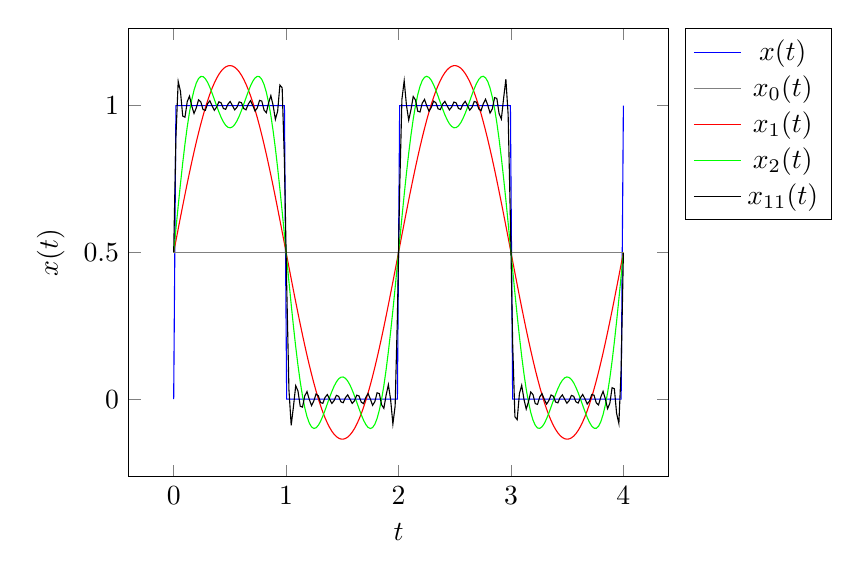
\begin{tikzpicture}
      \pgfmathdeclarefunction{p}{1}{%
        \pgfmathparse{(and(mod(#1,2)>0, mod(#1,2)<1))}%
      }
      \begin{axis}[domain=0:(4),samples=200, legend pos=outer north east ,xlabel={$t$},ylabel={$x(t)$}]
        \addplot[blue] {p(x)};
        \addplot[gray] {0.5}; % k=0
        \addplot[red] {0.5 + (2.0/3.1415)*cos(deg(3.1415*x - 1.571))}; % k=1
        \addplot[green] {0.5 + (2.0/3.1415)*cos(deg(3.1415*x - 1.571)) + (2.0/(3.1415*3))*cos(deg(3.1415*3*x - 1.571))}; % k=2
        %  \addplot[orange] {0.5 + (2.0/3.1415)*cos(deg(3.1415*x - 1.571)) + (2.0/(3.1415*3))*cos(deg(3.1415*3*x - 1.571)) + (2.0/(3.1415*5))*cos(deg(3.1415*5*x - 1.571))}; % k=5
        \addplot[black] {0.5 + (2.0/3.1415)*cos(deg(3.1415*x - 1.571))
          + (2.0/(3.1415*3))*cos(deg(3.1415*3*x - 1.571))
          + (2.0/(3.1415*5))*cos(deg(3.1415*5*x - 1.571))
          + (2.0/(3.1415*7))*cos(deg(3.1415*7*x - 1.571))
          + (2.0/(3.1415*9))*cos(deg(3.1415*9*x - 1.571))
          + (2.0/(3.1415*11))*cos(deg(3.1415*11*x - 1.571))
          + (2.0/(3.1415*13))*cos(deg(3.1415*13*x - 1.571))
          + (2.0/(3.1415*15))*cos(deg(3.1415*15*x - 1.571))
          + (2.0/(3.1415*17))*cos(deg(3.1415*17*x - 1.571))
          + (2.0/(3.1415*19))*cos(deg(3.1415*19*x - 1.571))
          + (2.0/(3.1415*21))*cos(deg(3.1415*21*x - 1.571))};
        %%                     + (2.0/(3.1415*23))*cos(deg(3.1415*23*x - 1.571))
        %                     + (2.0/(3.1415*25))*cos(deg(3.1415*25*x - 1.571))
        %                     + (2.0/(3.1415*27))*cos(deg(3.1415*27*x - 1.571))
        %                     + (2.0/(3.1415*29))*cos(deg(3.1415*29*x - 1.571))
        %                     + (2.0/(3.1415*31))*cos(deg(3.1415*31*x - 1.571))
        %                     + (2.0/(3.1415*33))*cos(deg(3.1415*33*x - 1.571))
        %                     + (2.0/(3.1415*35))*cos(deg(3.1415*35*x - 1.571))
        %                     + (2.0/(3.1415*37))*cos(deg(3.1415*37*x - 1.571)) 
        %                     + (2.0/(3.1415*39))*cos(deg(3.1415*39*x - 1.571)) 
        %                     + (2.0/(3.1415*41))*cos(deg(3.1415*41*x - 1.571)) 
        %                     + (2.0/(3.1415*43))*cos(deg(3.1415*43*x - 1.571)) 
        %                     + (2.0/(3.1415*45))*cos(deg(3.1415*45*x - 1.571)) 
        %                     + (2.0/(3.1415*47))*cos(deg(3.1415*47*x - 1.571)) 
        %                     + (2.0/(3.1415*49))*cos(deg(3.1415*49*x - 1.571)) 
        %                     + (2.0/(3.1415*51))*cos(deg(3.1415*51*x - 1.571)) 
        %                     + (2.0/(3.1415*53))*cos(deg(3.1415*53*x - 1.571)) 
        %                     + (2.0/(3.1415*55))*cos(deg(3.1415*55*x - 1.571))};

        \legend{$x(t)$,$x_0(t)$,$x_1(t)$,$x_2(t)$,$x_{11}(t)$}
      \end{axis}
    \end{tikzpicture}
  \end{center}
\fi

\newthought{The time derivative operator $\frac{d}{dt}$ has a very simple form for a Fourier series representation of a signal}.

We know that a Fourier series is a sum of complex sinusoidal signals. We also know that it is easy to differentiate this signal:
\begin{equation}
  \frac{d}{d t} c e^{i\omega t}=i\omega c e^{i\omega t}\,\,,
\end{equation}
where $c \in \mathbb{C}$ is a complex constant.

It is also relatively easy to see that the $n$th time derivative is:
\begin{equation}
  \frac{d^n}{dt^n}ce^{i\omega t} = (i\omega)^n c e^{i\omega t} \,\,.
\end{equation}
Thus, if $x(t)$ has a Fourier series representation
\begin{equation}
  x(t) = \sum_{k=-\infty}^{\infty} c_k e^{i\frac{2\pi}{T}kt}\,\,,
\end{equation}
then the $n$th time derivative has the following Fourier series representation:
\begin{align}
  \frac{d^n}{dt^n} x(t) & = \sum_{k=-\infty}^{\infty} i^n \left(\frac{2\pi k}{T}\right)^n c_k e^{i\frac{2\pi}{T}kt} \\
                        & = \sum_{k=-\infty}^{\infty} c^{(n)}_k e^{i\frac{2\pi}{T}kt} \,\,.
\end{align}
It is still a Fourier series, but with each Fourier coefficient modified in the following way:
\begin{equation}
  c_k^{(n)} := i^n \left(\frac{2\pi k}{T}\right)^n c_k \,\,.
  \label{eq:moddiff}
\end{equation}

Differentiation can be seen as a filtering operation on the signal. A filter is something
that modifies the amplitude and phase of the Fourier series coefficients in some way.
For example, a low-pass filtering operation would reduce the amplitudes of high frequency
coefficients relative to the amplitudes of the low frequency coefficients.
After a low-pass filtering operation, the ratio of low frequency coefficient amplitudes to
the high frequency coefficient amplitudes would be increased. A high pass filter on the other hand would do the opposite.

One thing to ask yourself is how does differentiation adjust the amplitude of each Fourier coefficient?
When taking the $n$th time derivative, what happens to the complex amplitudes at low angular
frequencies ($|2\pi k/T| < 1$)? What about high angular frequencies ($|2\pi k/T| > 1$)?
Hint, inspect how the coefficients defined in Equation \ref{eq:moddiff} are scaled.

The answer is that the magnitude of the low frequency Fourier coefficients are attenuated, and
high frequency ones are amplified. The DC component is completely removed as $2\pi k/T = 0$ for $k=0$.
Differentiation can therefore be viewed as a \emph{high-pass filtering} operation.

\newthought{The time shift operation $x(t-\tau)$ applied to a Fourier series representation} is also pretty handy.
Let's recall how a time shift affects a complex sinusoidal signal:
\begin{equation}
  x(t) = c e^{i\omega t} \,\,.
\end{equation}
If we apply a delay by $\tau$ to this signal $y(t) = x(t-\tau)$, we obtain:
\begin{align}
  y(t)  = c e^{i\omega (t-\tau)} =  e^{-i\omega \tau} c e^{i\omega t} = e^{-i\omega \tau} x(t) \,\,.
\end{align}
This means that a time delay by $\tau$ corresponds to a phase shift by $-\omega\tau$ for a complex sinusoidal signal.
We can apply this to a Fourier series, which is a sum of complex sinusoidal signals.

If the Fourier series representation of a signal is:
\begin{equation}
  x(t) = \sum_{k=-\infty}^{\infty} c_k e^{i\frac{2\pi}{T}kt} \,\,,
\end{equation}
then the Fourier series representation of a time shifted signal is:
\begin{align}
  x(t-\tau) & = \sum_{k=-\infty}^{\infty} \left(c_k e^{-i \frac{2\pi \tau}{T} k}\right) e^{i\frac{2\pi}{T}kt}\label{eq:time_shift_phasor} \\
            & =  \sum_{k=-\infty}^{\infty} c'_k e^{i\frac{2\pi}{T}kt}
\end{align}
where $c'_k$ is rotated on the complex plane in the clockwise direction by an angle of $2\pi k\tau/T$ with respect to $c_k$.

This means that if you know the Fourier series representation of a signal, you can easily modify the
complex amplitude $c_k$ of each Fourier coefficient to obtain the coefficients of the time shifted signal.

\newthought{What if a signal is not periodic, can we still form a spectral representation for a signal?}
Yes, we can. This investigation leads to the \emph{\index{continuous-time Fourier transform}{continuous-time Fourier transform}}.

Let's derive the continuous-time Fourier transform from the Fourier series. Pretty much all we'll need to do is
to study what happens when the fundamental period of the signal approaches infinity: $T\rightarrow \infty$.
We'll arrive with the result that introduces the Fourier transform, and the inverse Fourier transform, 
introducing, for the first time, this general spectral representation for continuous-time signals.

We start the derivation of the continuous-time Fourier transform with the definition of a Fourier series for a
function with period $T$. We'll denote by $\Delta \omega$ the spacing between frequency components.
The term $\Delta \omega$ also denotes the fundamental angular frequency of the periodic signal:
\begin{align}
  x_{T}(t) & = \sum_{k=-\infty}^{\infty} c_k e^{ik\Delta \omega t}  \,\,.
\end{align}
We can now add the definition of $c_k$ corresponding to the $k$th Fourier series coefficient using the synthesis equation:
\begin{align}
  x_{T}(t) & = \sum_{k=-\infty}^{\infty} \left[\frac{1}{T}\int_{-T/2}^{T/2} x_{T}(t) e^{-ik\Delta \omega t} dt\right]  e^{ik\Delta \omega t}  \,\,.
\end{align}
We then note that $1/T = \Delta \omega/2\pi$. This is the relationship between the fundamental period of
the signal and the fundamental angular frequency that we discussed in the beginning of this chapter.

We now obtain:
\begin{align}
  x_{T}(t) & = \frac{1}{2\pi}\sum_{k=-\infty}^{\infty} \left[\int_{-T/2}^{T/2} x_{T}(t) e^{-ik\Delta \omega t} dt\right]  e^{ik\Delta \omega t} \Delta \omega \\
           & = \frac{1}{2\pi}\sum_{k=-\infty}^{\infty} \hat{x}_{T}(k\Delta\omega)  e^{ik\Delta \omega t} \Delta \omega \,\,.
\end{align}
In this form, the equation is a Riemann sum approximation of an integral of a continuous function $\hat{x}_{T}(\omega)e^{-i\omega t}$.
\begin{figure}
  \begin{center}
    \begin{tikzpicture}
      \begin{axis}[width=13cm,height=6cm,ymin=-0,xmin=-3,ymax=1.8,xmax=3,  yticklabels={,,},
          xtick={-2,-1.5,-1,-0.5,0,0.5,1.0,1.5,2},
          xticklabels={$-4\Delta \omega$,$-3\Delta \omega$,$-2\Delta \omega$,$-\Delta \omega$,$0$,$\Delta \omega$,$2\Delta \omega$,$3\Delta \omega$,$4\Delta \omega$},
          xlabel=$\omega$, axis lines = center]

        \addplot+[ycomb] plot coordinates {(0.5,1) (1.0,0.8) (1.5,0.6) (2,0.5)};
        \addplot+[ycomb] plot coordinates {(-0.5,1) (-1.0,0.8) (-1.5,0.6) (-2,0.5)};
        \addplot+[ycomb] plot coordinates {(0.0, 1.4)};
        \node at (axis cs:-2.5,0.25) {$\cdots$};
        \node at (axis cs:2.5,0.25) {$\cdots$};
        \node at (axis cs:0.25,0.25) {$\Delta \omega$};


        %    \addplot [dimen] plot coordinates {(0.0,0.35) (0.5,0.35)};
        %    \addplot  plot coordinates {(0.0,0.35) (0.5,0.35)};
        \addplot[dimen]  plot coordinates {(0.0,0.35) (0.5,0.35)};
        \addplot[mark=none,color=gray] plot coordinates {(-2.25,0.5) (-1.75,0.5) (-1.75,0.6) (-1.25,0.6) (-1.25,0.8) (-.75,0.8) (-.75,1) (-.25,1) (-.25,1.4) (.25,1.4) (.25,1) (.75,1) (.75,0.8) (1.25,0.8) (1.25,0.6) (1.75,0.6) (1.75,0.5) (2.25,0.5)} ;

        \addplot[mark=none,color=black] plot [smooth,tension=0.1] coordinates {(-2.,0.5) (-1.5,0.6) (-1,0.8) (-.5,1) (0,1.4) (.5,1.) (1,0.8) (1.5,0.6) (2,0.5) } ;

        \node at (axis cs:0.0,1.5) [above right, font={\footnotesize}]{$c_0$};
        \node at (axis cs:0.5,1.1) [above, font={\footnotesize}]{$c_1$};
        \node at (axis cs:1.0,0.9) [above, font={\footnotesize}]{$c_2$};
        \node at (axis cs:1.5,0.7) [above, font={\footnotesize}]{$c_3$};
        \node at (axis cs:2.0,0.6) [above, font={\footnotesize}]{$c_4$};

        \node at (axis cs:-0.5,1.1) [above, font={\footnotesize}]{$c_{-1}$};
        \node at (axis cs:-1.0,0.9) [above, font={\footnotesize}]{$c_{-2}$};
        \node at (axis cs:-1.5,0.7) [above, font={\footnotesize}]{$c_{-3}$};
        \node at (axis cs:-2.0,0.6) [above, font={\footnotesize}]{$c_{-4}$};
      \end{axis}
    \end{tikzpicture}
  \end{center}
  \caption{A depiction of how the Fourier series can be seen as a Riemann sum approximation of an integral of a continuous function.}
\end{figure}

We now inspect the case where $T\rightarrow \infty$. When the period of the
function $x_{T}(t)$ approaches infinity,
we drop the subscript $T$ in the notation and denote it with $x(t)$.
The Riemann sum then approaches the following integral
equation ($\Delta\omega \rightarrow d\omega$, $k\Delta\omega \rightarrow \omega$):
\begin{align}
  \lim_{T\rightarrow \infty} x_{T}(t) & = \lim_{T\rightarrow \infty}\frac{1}{2\pi} \sum_{k=-\infty}^{\infty} \hat{x}_{T}(k\Delta \omega) e^{ik\Delta \omega t}\Delta\omega \\
                                      & =\frac{1}{2\pi}\int_{-\infty}^{\infty} \left[\int_{-\infty}^{\infty} x(t) e^{-i\omega t} dt\right] e^{i\omega t}d\omega            \\
                                      & = \frac{1}{2\pi} \int_{-\infty}^{\infty} \hat{x}(\omega) e^{i\omega t}d\omega                                                      \\
                                      & = x(t) \,\,.
\end{align}
This integral is known as the inverse Fourier transform. It allows us to go from a continuous function $\hat{x}(\omega)$,
which is the continuous spectral representation of the signal, to the time domain signal $x(t)$.

The innermost integral that allows us to obtain $\hat{x}(\omega)$ from the continuous-time signal $x(t)$ is:
\begin{align}
  \hat{x}(\omega) & = \int_{-\infty}^{\infty} x(t) e^{-i\omega t} dt \,\,.
\end{align}
This is the forward Fourier transform.

\newthought{The forward Fourier transform} is defined as:

\begin{equation}
  \boxed{
    \hat{x}(\omega) = \int_{-\infty}^{\infty} x(t) e^{-i\omega t}dt
  } \,\,.
\end{equation}

\newthought{The inverse Fourier transform} is defined as:

\begin{equation}
  \boxed{
    x(t) = \frac{1}{2\pi}\int_{-\infty}^{\infty} \hat{x}(\omega) e^{i\omega t}d\omega
  } \,\,.
\end{equation}
Just as the Fourier series, the continuous-time Fourier transform is in most practical cases invertible.

We'll use the following notation to indicate Fourier transform pairs:
\begin{equation}
  \boxed{
    x(t) \xleftrightarrow{\mathcal{F}} \hat{x}(\omega)
  } \,\,.
\end{equation}
We'll return to the Fourier transform later and show that the Fourier series is a special case of the Fourier transform!

\section{The spectrum of an audio signal}

The Python program in Listing \ref{lst:audio_spec} shows how to use the Fast Fourier Transform (FFT)
command in Python to analyze an audio signal for its spectral contents.
The output of this program is shown in Figure \ref{fig:audio_spec}.

The FFT algorithm is used to evaluate a discrete-time Fourier transform.
This operation is mathematically defined as follows:
\begin{equation}
  c[k] = \sum_{t=0}^{N-1} x[t] e^{-i\frac{2\pi}{N}kt} \,\,.
\end{equation}
Here $c[k]$ is the complex amplitude corresponding to a spectral component with angular frequency $\omega_k = 2\pi k/(T_s N)$, where $T_s=1/f_s$ is the sample-spacing, which is the inverse of the sample-rate of the signal.

You can think of an FFT as a discrete-time equivalent of the Fourier series analysis equation, 
which finds the Fourier series coefficients for a periodic discrete-time signal. 
We will cover the discrete Fourier transform and discrete-time signals in more detail later on, 
I just wanted to already expose you to the FFT algorithm at this point.

\lstinputlisting[language=Python, caption={\texttt{013\_audio\_spec/audio\_spec.py}}, label=lst:audio_spec]{code/013_audio_spec/audio_spec.py}

\begin{figure}
  \begin{center}
    %\includegraphics[width=0.67\textwidth]{ch03/guitar_str.png}
    \includegraphics[width=\textwidth]{code/013_audio_spec/audio_spec.png}
  \end{center}
  \caption{The spectral components of an audio signal (guitar string plucked). Left: time domain signal $x(t)$, Right: The magnitude of the spectral components in decibel scale: $10\log_{10}(|c_k|^2)$.}
  \label{fig:audio_spec}
\end{figure}
